%\addtocontents{toc}{\setlength\cftchapternumwidth{1em}}
%\renewcommand\thechapter{}


\chapter{Trigger scale factors}
%\renewcommand{\thechapter}{A}
\label{app:TriggerSF}



The trigger scale factors measured as a function of lepton \pt, using the dataset collected by \Etmis\ triggers and \WZ\ simulation, after a 3 lepton and jets selection, in the Z mass window. All corrections to simulation are applied.



\begin{table}[htbp]
	\centering
	\caption{Trigger efficiencies on data events selected with \Etmis\ triggers and \WZ\ simulation for all leptonic channels together. The unweighed number of events is quoted. When there are no events passing the cuts, it is indicated with N/A. The uncertainties are statistical uncertainties.}
	\begin{tabular}{c|c|c|c|c}
		\toprule
		ALL CHANNEL & \multicolumn{2}{c|}{data} & \multicolumn{2}{c}{WZ simulations} \\ 
		& Efficiency & unc. & Efficiency & unc. \\
		\midrule 
		3 lep,  at least one jet & 117/118 = 99.15 \% & 12.94\% & 18047/18055 = 99.96\%  & 1.05\% \\ 
		\hline 
		\STSR & 6/6 = 100.00\% & 57.74\% & 1541/1541 = 100.00\% & 3.60\% \\ 
		\hline 
		\TTSR & 26/27 = 96.30\% & 26.46\% & 1791/1792 = 99.94\% & 3.34\% \\ 
		\hline 
		\WZCR & 69/69 = 100.00 \% & 17.03\% & 14405/14412=99.95\% & 1.18\% \\ 
		\bottomrule 
	\end{tabular} 
\end{table}	
\begin{table}[htbp]
	\centering
	\caption{Trigger efficiencies on data events selected with \Etmis\ triggers and \WZ\ simulation for \mumumu\ leptonic channel together. The unweighed number of events is quoted. When there are no events passing the cuts, it is indicated with N/A. The uncertainties are statistical uncertainties.}
	\begin{tabular}{c|c|c|c|c}
		\toprule 
		\mumumu\ CHANNEL & \multicolumn{2}{c|}{data} & \multicolumn{2}{c}{\WZ\ simulations} \\
		& Efficiency & unc. & Efficiency & unc. \\ 
		\midrule 
		3 lep,  at least one jet & 40/40 = 100.00 \% & 22.36 \% & 7814/7814 = 100.00\%  & 1.60\% \\ 
		\hline 
		\STSR & N/A & N/A & 687/687 = 100\% & 5.40\% \\ 
		\hline 
		\TTSR & 13/13 = 100.00\% & 39.22\% &763/763 = 100.00\% & 5.12\% \\ 
		\hline 
		\WZCR & 22/22 = 100.00 \% & 30.15\% & 6238/6238=100.00\% & 1.79\% \\ 
		\bottomrule
	\end{tabular} 
\end{table}	
\begin{table}[htbp]
	\centering
	\caption{Trigger efficiencies on data events selected with \Etmis\ triggers and \WZ\ simulation for \eee\ leptonic channel together. The unweighed number of events is quoted. When there are no events passing the cuts, it is indicated with N/A. The uncertainties are statistical uncertainties.}

	\begin{tabular}{c|c|c|c|c}
		\toprule 
		\eee\ CHANNEL & \multicolumn{2}{c|}{data} & \multicolumn{2}{c}{WZ simulations} \\ 
		& Efficiency & unc. & Efficiency & unc. \\
		\midrule
		3 lep,  at least one jet & 20/21 = 95.24\%  & 29.76\% & 2211/2215 = 99.82 \% & 3.00\%  \\ 
		\hline 
		\STSR & 4/4 = 100.00\% & 70.71\% & 176/176 = 100.00\% & 10.66\% \\ 
		\hline 
		\TTSR & 2/3 = 66.67\% & 60.86\% & 242/242 = 100.00\% & 9.09\% \\ 
		\hline 
		\WZCR & 14/14 = 100.00 \% & 37.80\% & 1744/1748=99.77\% & 3.38\% \\ 
		\bottomrule
	\end{tabular} 
\end{table}
\begin{table}[htbp]
	\centering
	\caption{Trigger efficiencies on data events selected with \Etmis\ triggers and \WZ\ simulation for \eemu\ leptonic channel together. The unweighed number of events is quoted. When there are no events passing the cuts, it is indicated with N/A. The uncertainties are statistical uncertainties.}

	\begin{tabular}{c|c|c|c|c}
		\toprule
		\eemu\ CHANNEL & \multicolumn{2}{c|}{data} & \multicolumn{2}{c}{WZ simulations} \\ 
		& Efficiency & unc. & Efficiency & unc. \\
		\midrule
		3 lep,  at least one jet & 32/32 = 100.00 \% & 25.00 \% & 3116/3118 = 99.94\%  & 2.53\% \\ 
		\hline 
		\STSR & 1/1 = 100.00\%& 141.42\% & 255/255 = 100\% & 8.86\% \\ 
		\hline 
		\TTSR & 9/9 = 100.00\% & 47.14\% &291/291 = 100.00\% & 8.29\% \\ 
		\hline 
		\WZCR & 14/14 = 100.00 \% & 37.80\% & 2529/2531=99.92\% & 2.81\% \\ 
		\bottomrule
	\end{tabular} 
\end{table}	
\begin{table}[htbp]
	\centering
	\caption{Trigger efficiencies on data events selected with \Etmis\ triggers and \WZ\ simulation for \emumu\ leptonic channel together. The unweighed number of events is quoted. When there are no events passing the cuts, it is indicated with N/A. The uncertainties are statistical uncertainties.}

	\begin{tabular}{c|c|c|c|c}
		\toprule 
		\emumu\ CHANNEL & \multicolumn{2}{c|}{data} & \multicolumn{2}{c}{WZ simulations} \\ 
		& Efficiency & unc. & Efficiency & unc. \\
		\midrule
		3 lep,  at least one jet & 25/25 = 100.00\%  & 28.28\% & 4906/4908 = 99.96 \% & 2.02\%  \\ 
		\hline 
		\STSR & 1/1 = 100.00\% &141.42\% & 423/423 = 100.00\% & 6.88\% \\ 
		\hline 
		\TTSR & 2/2 = 100.00\% & 100.00\% & 495/496 = 99.80\% & 6.34\% \\ 
		\hline 
		\WZCR & 19/19 = 100.00 \% & 32.44\% & 3894/3895 =99.97\% & 2.27\% \\ 
		\bottomrule 
	\end{tabular} 
	\label{tab:trigSF}
\end{table}
\begin{comment}

\begin{figure}[tb]
	[In function of lepton \pt]{
		\includegraphics[width=0.48\textwidth]{Appendix/Figures/trigger/Triggereff/1e2mu/triggeff_1e2muhistPt.png}
		\label{image:triggeff_1e2muhistPt.png}
	}
	[In function of 2nd leading lepton in \pt]{
		\includegraphics[width=0.48\textwidth]{Appendix/Figures/trigger/Triggereff/1e2mu/triggeff_1e2muhistPt_2ndleadinglep.png}
		\label{image:triggeff_1e2muhistPt_2ndleadinglep.png}
	}
	\newline
	[In function of 3d leading lepton in \pt]{
		\includegraphics[width=0.48\textwidth]{Appendix/Figures/trigger/Triggereff/1e2mu/triggeff_1e2muhistPt_3dleadinglep.png}
		\label{image:triggeff_1e2muhistPt_3dleadinglep.png}
	}
	[In function of leading lepton in \pt]{
		\includegraphics[width=0.48\textwidth]{Appendix/Figures/trigger/Triggereff/1e2mu/triggeff_1e2muhistPt_leadinglep.png}
		\label{image:triggeff_1e2muhistPt_leadinglep.png}
	}
	\caption{The trigger efficiencies measured as a function of lepton \pt, using the dataset collected by \Etmis\ triggers and \WZ\ simulation, after a 3 lepton and jets selection, in the Z mass window. All corrections to simulation are applied. 1e2$\mu$ channel.}
	\label{image:FigurestriggerTriggereff1e2mu}
\end{figure}

\begin{figure}[tb]
	[In function of lepton \pt]{
		\includegraphics[width=0.48\textwidth]{Appendix/Figures/trigger/Triggereff/2e1mu/triggeff_2e1muhistPt.png}
		\label{image:triggeff_2e1muhistPt.png}
	}
	[In function of 2nd leading lepton in \pt]{
		\includegraphics[width=0.48\textwidth]{Appendix/Figures/trigger/Triggereff/2e1mu/triggeff_2e1muhistPt_2ndleadinglep.png}
		\label{image:triggeff_2e1muhistPt_2ndleadinglep.png}
	}
	\newline
	[In function of 3d leading lepton in \pt]{
		\includegraphics[width=0.48\textwidth]{Appendix/Figures/trigger/Triggereff/2e1mu/triggeff_2e1muhistPt_3dleadinglep.png}
		\label{image:triggeff_2e1muhistPt_3dleadinglep.png}
	}
	[In function of leading lepton in \pt]{
		\includegraphics[width=0.48\textwidth]{Appendix/Figures/trigger/Triggereff/2e1mu/triggeff_2e1muhistPt_leadinglep.png}
		\label{image:triggeff_2e1muhistPt_leadinglep.png}
	}
	\caption{The trigger efficiencies measured as a function of lepton \pt, using the dataset collected by \Etmis\ triggers and \WZ\ simulation, after a 3 lepton and jets selection, in the Z mass window. All corrections to simulation are applied. 2e1$\mu$ channel.}
	\label{image:FigurestriggerTriggereff2e1mu}
\end{figure}

\begin{figure}[tb]
	[In function of lepton \pt]{
		\includegraphics[width=0.48\textwidth]{Appendix/Figures/trigger/Triggereff/3e/triggeff_3ehistPt.png}
		\label{image:triggeff_3ehistPt.png}
	}
	[In function of 2nd leading lepton in \pt]{
		\includegraphics[width=0.48\textwidth]{Appendix/Figures/trigger/Triggereff/3e/triggeff_3ehistPt_2ndleadinglep.png}
		\label{image:triggeff_3ehistPt_2ndleadinglep.png}
	}
	\newline
	[In function of 3d leading lepton in \pt]{
		\includegraphics[width=0.48\textwidth]{Appendix/Figures/trigger/Triggereff/3e/triggeff_3ehistPt_3dleadinglep.png}
		\label{image:triggeff_3ehistPt_3dleadinglep.png}
	}
	[In function of leading lepton in \pt]{
		\includegraphics[width=0.48\textwidth]{Appendix/Figures/trigger/Triggereff/3e/triggeff_3ehistPt_leadinglep.png}
		\label{image:triggeff_3ehistPt_leadinglep.png}
	}
	\caption{The trigger efficiencies measured as a function of lepton \pt, using the dataset collected by \Etmis\ triggers and \WZ\ simulation, after a 3 lepton and jets selection, in the Z mass window. All corrections to simulation are applied. 3e channel.}
	\label{image:FigurestriggerTriggereff3e}
\end{figure}

\begin{figure}[tb]
	[In function of lepton \pt]{
		\includegraphics[width=0.48\textwidth]{Appendix/Figures/trigger/Triggereff/3mu/triggeff_3muhistPt.png}
		\label{image:triggeff_3muhistPt.png}
	}
	[In function of 2nd leading lepton in \pt]{
		\includegraphics[width=0.48\textwidth]{Appendix/Figures/trigger/Triggereff/3mu/triggeff_3muhistPt_2ndleadinglep.png}
		\label{image:triggeff_3muhistPt_2ndleadinglep.png}
	}
	\newline
	[In function of 3d leading lepton in \pt]{
		\includegraphics[width=0.48\textwidth]{Appendix/Figures/trigger/Triggereff/3mu/triggeff_3muhistPt_3dleadinglep.png}
		\label{image:triggeff_3muhistPt_3dleadinglep.png}
	}
	[In function of leading lepton in \pt]{
		\includegraphics[width=0.48\textwidth]{Appendix/Figures/trigger/Triggereff/3mu/triggeff_3muhistPt_leadinglep.png}
		\label{image:triggeff_3muhistPt_leadinglep.png}
	}
	\caption{The trigger efficiencies measured as a function of lepton \pt, using the dataset collected by \Etmis\ triggers and \WZ\ simulation, after a 3 lepton and jets selection, in the Z mass window. All corrections to simulation are applied. 3$\mu$ channel.}
	\label{image:FigurestriggerTriggereff3mu}
\end{figure}

\begin{figure}[tb]
	[In function of lepton \pt]{
		\includegraphics[width=0.48\textwidth]{Appendix/Figures/trigger/Triggereff/all/triggeff_allhistPt.png}
		\label{image:triggeff_allhistPt.png}
	}
	[In function of 2nd leading lepton in \pt]{
		\includegraphics[width=0.48\textwidth]{Appendix/Figures/trigger/Triggereff/all/triggeff_allhistPt_2ndleadinglep.png}
		\label{image:triggeff_allhistPt_2ndleadinglep.png}
	}
	\newline
	[In function of 3d leading lepton in \pt]{
		\includegraphics[width=0.48\textwidth]{Appendix/Figures/trigger/Triggereff/all/triggeff_allhistPt_3dleadinglep.png}
		\label{image:triggeff_allhistPt_3dleadinglep.png}
	}
	[In function of leading lepton in \pt]{
		\includegraphics[width=0.48\textwidth]{Appendix/Figures/trigger/Triggereff/all/triggeff_allhistPt_leadinglep.png}
		\label{image:triggeff_allhistPt_leadinglep.png}
	}
	\caption{The trigger efficiencies measured as a function of lepton \pt, using the dataset collected by \Etmis\ triggers and \WZ\ simulation, after a 3 lepton and jets selection, in the Z mass window. All corrections to simulation are applied. All channel.}
	\label{image:FigurestriggerTriggereffall}
\end{figure}

\begin{figure}[tb]
	[In function of lepton \pt]{
		\includegraphics[width=0.48\textwidth]{Appendix/Figures/trigger/ScaleFactors/1e2mu/SF_trigger_1e2muhistPt.png}
		\label{image:1e2muhistPt.png}
	}
	[In function of 2nd leading lepton in \pt]{
		\includegraphics[width=0.48\textwidth]{Appendix/Figures/trigger/ScaleFactors/1e2mu/SF_trigger_1e2muhistPt_2ndleadinglep.png}
		\label{image:1e2muhistPt_2ndleadinglep.png}
	}
	\newline
	[In function of 3d leading lepton in \pt]{
		\includegraphics[width=0.48\textwidth]{Appendix/Figures/trigger/ScaleFactors/1e2mu/SF_trigger_1e2muhistPt_3dleadinglep.png}
		\label{image:1e2muhistPt_3dleadinglep.png}
	}
	[In function of leading lepton in \pt]{
		\includegraphics[width=0.48\textwidth]{Appendix/Figures/trigger/ScaleFactors/1e2mu/SF_trigger_1e2muhistPt_leadinglep.png}
		\label{image:1e2muhistPt_leadinglep.png}
	}
	\caption{The trigger scale factors measured as a function of lepton \pt, using the dataset collected by \Etmis\ triggers and \WZ\ simulation, after a 3 lepton and jets selection, in the Z mass window. All corrections to simulation are applied. 1e2$\mu$ channel.}
	\label{image:FigurestriggerScaleFactors1e2mu}
\end{figure}

\begin{figure}[tb]
	[In function of lepton \pt]{
		\includegraphics[width=0.48\textwidth]{Appendix/Figures/trigger/ScaleFactors/2e1mu/SF_trigger_2e1muhistPt.png}
		\label{image:2e1muhistPt.png}
	}
	[In function of 2nd leading lepton in \pt]{
		\includegraphics[width=0.48\textwidth]{Appendix/Figures/trigger/ScaleFactors/2e1mu/SF_trigger_2e1muhistPt_2ndleadinglep.png}
		\label{image:2e1muhistPt_2ndleadinglep.png}
	}
	\newline
	[In function of 3d leading lepton in \pt]{
		\includegraphics[width=0.48\textwidth]{Appendix/Figures/trigger/ScaleFactors/2e1mu/SF_trigger_2e1muhistPt_3dleadinglep.png}
		\label{image:2e1muhistPt_3dleadinglep.png}
	}
	[In function of leading lepton in \pt]{
		\includegraphics[width=0.48\textwidth]{Appendix/Figures/trigger/ScaleFactors/2e1mu/SF_trigger_2e1muhistPt_leadinglep.png}
		\label{image:2e1muhistPt_leadinglep.png}
	}
	\caption{The trigger scale factors measured as a function of lepton \pt, using the dataset collected by \Etmis\ triggers and \WZ\ simulation, after a 3 lepton and jets selection, in the Z mass window. All corrections to simulation are applied. 2e1$\mu$ channel.}
	\label{image:FigurestriggerScaleFactors2e1mu}
\end{figure}

\begin{figure}[tb]
	[In function of lepton \pt]{
		\includegraphics[width=0.48\textwidth]{Appendix/Figures/trigger/ScaleFactors/3e/SF_trigger_3ehistPt.png}
		\label{image:3ehistPt.png}
	}
	[In function of 2nd leading lepton in \pt]{
		\includegraphics[width=0.48\textwidth]{Appendix/Figures/trigger/ScaleFactors/3e/SF_trigger_3ehistPt_2ndleadinglep.png}
		\label{image:3ehistPt_2ndleadinglep.png}
	}
	\newline
	[In function of 3d leading lepton in \pt]{
		\includegraphics[width=0.48\textwidth]{Appendix/Figures/trigger/ScaleFactors/3e/SF_trigger_3ehistPt_3dleadinglep.png}
		\label{image:3ehistPt_3dleadinglep.png}
	}
	[In function of leading lepton in \pt]{
		\includegraphics[width=0.48\textwidth]{Appendix/Figures/trigger/ScaleFactors/3e/SF_trigger_3ehistPt_leadinglep.png}
		\label{image:3ehistPt_leadinglep.png}
	}
	\caption{The trigger scale factors measured as a function of lepton \pt, using the dataset collected by \Etmis\ triggers and \WZ\ simulation, after a 3 lepton and jets selection, in the Z mass window. All corrections to simulation are applied. 3e channel.}
	\label{image:FigurestriggerScaleFactors3e}
\end{figure}

\begin{figure}[tb]
	[In function of lepton \pt]{
		\includegraphics[width=0.48\textwidth]{Appendix/Figures/trigger/ScaleFactors/3mu/SF_trigger_3muhistPt.png}
		\label{image:3muhistPt.png}
	}
	[In function of 2nd leading lepton in \pt]{
		\includegraphics[width=0.48\textwidth]{Appendix/Figures/trigger/ScaleFactors/3mu/SF_trigger_3muhistPt_2ndleadinglep.png}
		\label{image:3muhistPt_2ndleadinglep.png}
	}
	\newline
	[In function of 3d leading lepton in \pt]{
		\includegraphics[width=0.48\textwidth]{Appendix/Figures/trigger/ScaleFactors/3mu/SF_trigger_3muhistPt_3dleadinglep.png}
		\label{image:3muhistPt_3dleadinglep.png}
	}
	[In function of leading lepton in \pt]{
		\includegraphics[width=0.48\textwidth]{Appendix/Figures/trigger/ScaleFactors/3mu/SF_trigger_3muhistPt_leadinglep.png}
		\label{image:3muhistPt_leadinglep.png}
	}
	\caption{The trigger scale factors measured as a function of lepton \pt, using the dataset collected by \Etmis\ triggers and \WZ\ simulation, after a 3 lepton and jets selection, in the Z mass window. All corrections to simulation are applied. 3$\mu$ channel.}
	\label{image:FigurestriggerScaleFactors3mu}
\end{figure}

\begin{figure}[tb]
	[In function of lepton \pt]{
		\includegraphics[width=0.48\textwidth]{Appendix/Figures/trigger/ScaleFactors/all/SF_trigger_allhistPt.png}
		\label{image:allhistPt.png}
	}
	[In function of 2nd leading lepton in \pt]{
		\includegraphics[width=0.48\textwidth]{Appendix/Figures/trigger/ScaleFactors/all/SF_trigger_allhistPt_2ndleadinglep.png}
		\label{image:allhistPt_2ndleadinglep.png}
	}
	\newline
	[In function of 3d leading lepton in \pt]{
		\includegraphics[width=0.48\textwidth]{Appendix/Figures/trigger/ScaleFactors/all/SF_trigger_allhistPt_3dleadinglep.png}
		\label{image:allhistPt_3dleadinglep.png}
	}
	[In function of leading lepton in \pt]{
		\includegraphics[width=0.48\textwidth]{Appendix/Figures/trigger/ScaleFactors/all/SF_trigger_allhistPt_leadinglep.png}
		\label{image:allhistPt_leadinglep.png}
	}
	\caption{The trigger scale factors measured as a function of lepton \pt, using the dataset collected by \Etmis\ triggers and \WZ\ simulation, after a 3 lepton and jets selection, in the Z mass window. All corrections to simulation are applied. All channel.}
	\label{image:FigurestriggerScaleFactorsall}
\end{figure}
\end{comment}

\chapter{Dilepton controlplots}
\label{app:controldilep}


\chapter{Statistical independent regions}
\label{app:tablestr}
\begin{landscape}
	\begin{table}
		\begin{center}
			\begin{tabular} {|l| c|c|c|c|c|c|c|c|c|}
				\hline 
				& \STSR & \TTSR & \WZCR & \TTCR & \STCR & $Tr_{\WZCR \rightarrow \STSR}$ & $Tr_{\WZCR \rightarrow \TTSR}$ & $Tr_{\TTCR \rightarrow \TTSR}$ & $Tr_{\STCR \rightarrow \STSR}$  \\ 
				\hline 
				\textbf{FCNC tZu} & 3.9 $\pm $0.0 & 11.2 $\pm $0.0 & 7.3 $\pm $0.0 & 0.6 $\pm $0.0 & 0.3 $\pm $0.0 & 0.22 $\pm $0.00 & 0.46 $\pm $0.00 & $-$  & $-$  \\  
				\textbf{FCNC tZc} & 14.1 $\pm $0.1 & 30.9 $\pm $0.1 & 15.5 $\pm $0.1 & 1.7 $\pm $0.0 & 1.2 $\pm $0.0 & 0.39 $\pm $0.01 & 0.76 $\pm $0.01 & $-$  & $-$  \\  
				\textbf{DY } & -4.6 $\pm $21.7 & 22.3 $\pm $14.3 & 136.9 $\pm $48.5 & -14.0 $\pm $22.2 & -15.9 $\pm $11.3 & 0.08 $\pm $0.09 & 0.10 $\pm $0.10 & $-$  & $-$  \\  
				\textbf{ttbar} & 13.1 $\pm $2.5 & 9.7 $\pm $2.1 & 8.5 $\pm $1.9 & 22.3 $\pm $3.1 & 33.7 $\pm $3.8 & 0.54 $\pm $0.31 & 0.70 $\pm $0.31 & 0.33 $\pm $0.00 & 0.33 $\pm $0.00 \\  
				\textbf{DD fake} & 62.0 $\pm $7.9 & 63.0 $\pm $7.9 & 204.0 $\pm $14.3 & 41.0 $\pm $6.4 & 56.0 $\pm $7.5 & $-$  & $-$  & $-$  & $-$  \\  
				\textbf{WZ+jets} & 60.9 $\pm $1.6 & 83.0 $\pm $1.7 & 552.7 $\pm $4.6 & 11.9 $\pm $0.6 & 8.5 $\pm $0.6 & 0.10 $\pm $0.00 & 0.15 $\pm $0.00 & $-$  & $-$  \\  
				\textbf{tZq} & 8.0 $\pm $0.2 & 16.9 $\pm $0.2 & 7.3 $\pm $0.2 & 2.2 $\pm $0.1 & 1.0 $\pm $0.1 & 0.36 $\pm $0.02 & 0.67 $\pm $0.03 & $-$  & $-$  \\  
				\textbf{ttZ} & 3.5 $\pm $0.3 & 42.5 $\pm $0.9 & 9.6 $\pm $0.5 & 6.8 $\pm $0.4 & 0.5 $\pm $0.1 & 0.14 $\pm $0.02 & 0.61 $\pm $0.05 & $-$  & $-$  \\  
				\textbf{ZZ} & 4.6 $\pm $0.1 & 4.8 $\pm $0.1 & 46.2 $\pm $0.3 & 0.8 $\pm $0.0 & 0.6 $\pm $0.0 & 0.10 $\pm $0.00 & 0.13 $\pm $0.00 & $-$  & $-$  \\  
				\textbf{other} & 1.2 $\pm $0.3 & 5.6 $\pm $0.3 & 6.8 $\pm $0.5 & 7.5 $\pm $0.7 & 2.4 $\pm $0.5 & 0.16 $\pm $0.03 & 0.30 $\pm $0.03 & $-$  & $-$  \\  
				\hline 
			\end{tabular}
			\caption{Event yields:  All channel.The last three columns represent the transfer factors that have to be applied.}
		\end{center}
	\end{table}
	
	
\end{landscape}
\chapter{Details about the BDTs}
\label{app:BDTtechnics}
The boosted decision are trained without the \NPL\ background.
\section*{Boosted Decision Tree Factory in \STSR}
In the TMVA factory, 
\begin{description}
	\item[]\textcolor{ForestGreen}{
		TMVA::Factory(bdt\_type.Data(), output\_file, \\
		''!V:!Silent:Color:!DrawProgressBar:Transformations=I:AnalysisType=Classification``)},
\end{description}
the trees are trained and tested by 
\begin{description}
	\item[] \textcolor{ForestGreen}{factory$\rightarrow$PrepareTrainingAndTestTree( mycuts, mycutb,\\ ''nTrain\_Signal=0:nTrain\_Background=0:SplitMode=Random:NormMode=NumEvents:!V``)},
\end{description}
and the BDT is constructed as:
\begin{description}
	\item[] \textcolor{ForestGreen}{factory$\rightarrow$BookMethod( TMVA::Types::kBDT,method\_title.Data(),\\''!H:!V:NTrees=25:MinNodeSize=15\%:BoostType=Grad:Shrinkage=0.3:\\SeparationType=GiniIndex:nCuts=15:MaxDepth=3:NegWeightTreatment=Pray:\\PruneMethod=NoPruning:UseBaggedBoost:BaggedSampleFrcation=0.5`` )}.
\end{description}


\section*{Boosted Decision Tree Factory in \TTSR}
In the TMVA factory, 
\begin{description}
	\item[]\textcolor{ForestGreen}{
		TMVA::Factory(bdt\_type.Data(), output\_file, \\
		''!V:!Silent:Color:!DrawProgressBar:Transformations=I;D;P;G,D:AnalysisType=Classification``)},
\end{description}
the trees are trained and tested by 
\begin{description}
	\item[] \textcolor{ForestGreen}{factory$\rightarrow$PrepareTrainingAndTestTree( mycuts, mycutb,\\ ''nTrain\_Signal=0:nTrain\_Background=0:SplitMode=Random:NormMode=NumEvents:!V``)},
\end{description}
and the BDT is constructed as:
\begin{description}
	\item[] \textcolor{ForestGreen}{factory$\rightarrow$BookMethod( TMVA::Types::kBDT,method\_title.Data(),\\''!H:!V:NTrees=225:MinNodeSize=5\%:BoostType=Grad:Shrinkage=0.2:\\UseBaggedBoost:BaggedSampleFraction=0.8:SeparationType=GiniIndex:nCuts=15:\\MaxDepth=3:NegWeightTreatment=Pray`` )}.
\end{description}

\section*{BDT control distributions}

\begin{figure}[htbp]
	\includegraphics[width=0.48\textwidth]{6_Search/Figures/MVAtechnics/toppairzct/eee/CorrelationMatrixB.png}
	\includegraphics[width=0.48\textwidth]{6_Search/Figures/MVAtechnics/toppairzct/eee/CorrelationMatrixS.png}
	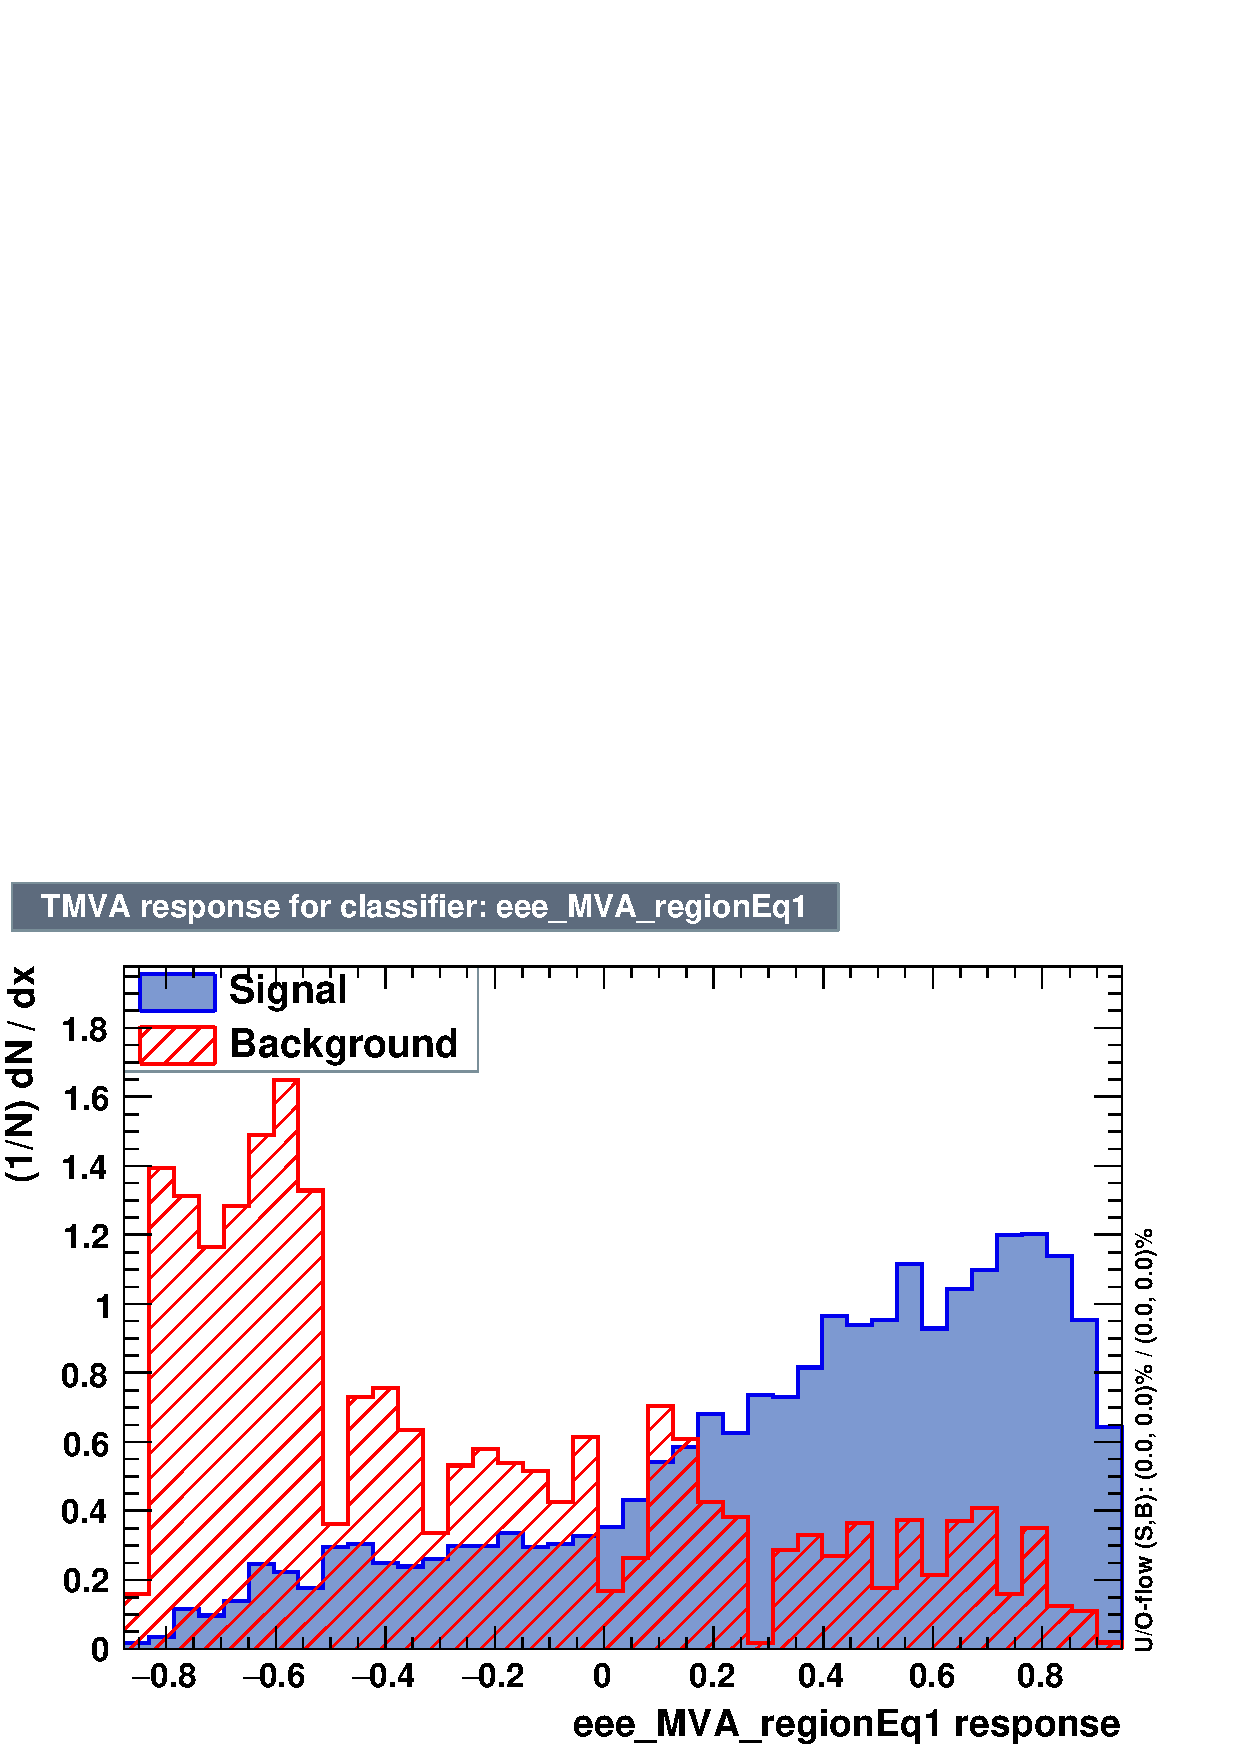
\includegraphics[width=0.48\textwidth]{6_Search/Figures/MVAtechnics/toppairzct/eee/mva_eee_MVA_regionEq1.png}
	\includegraphics[width=0.48\textwidth]{6_Search/Figures/MVAtechnics/toppairzct/eee/rejBvsS.png}
	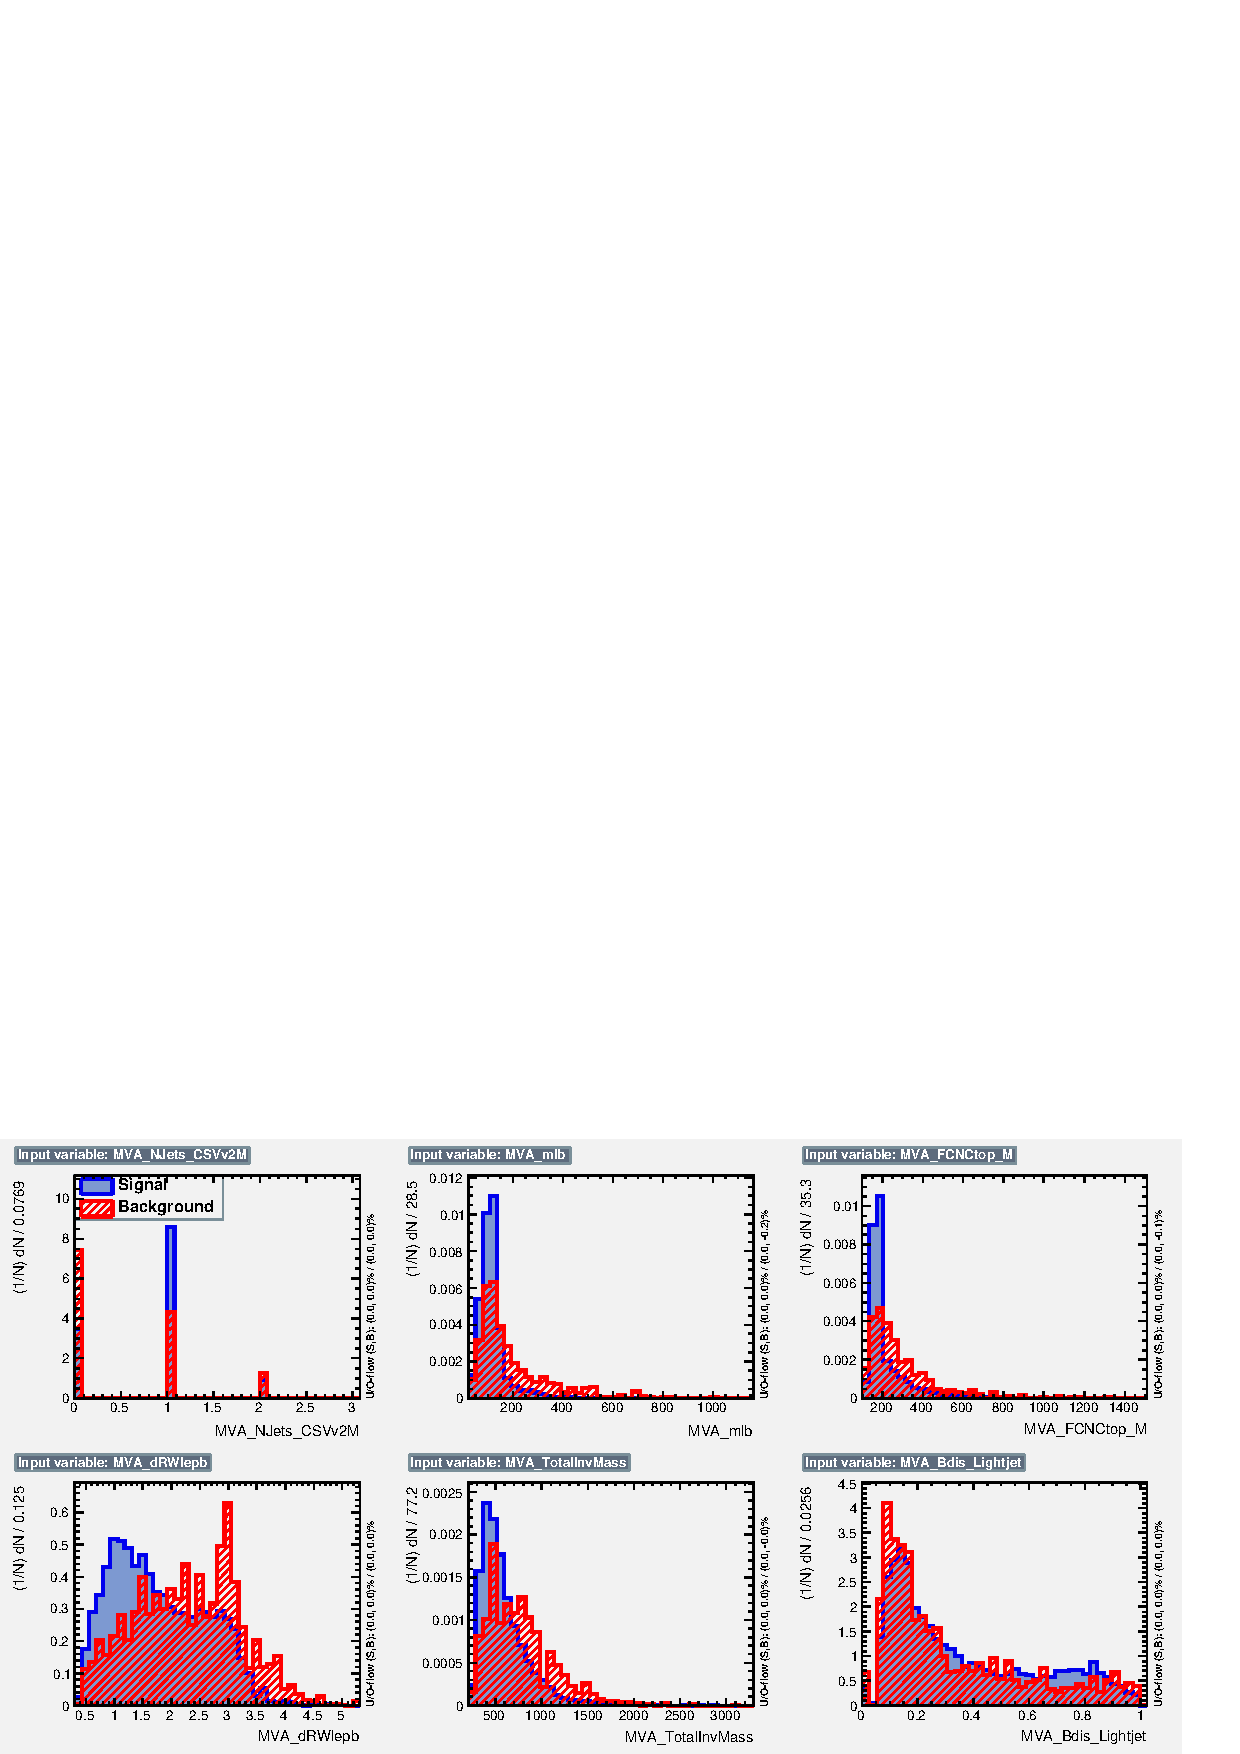
\includegraphics[width=0.48\textwidth]{6_Search/Figures/MVAtechnics/toppairzct/eee/variables_id_c1.png}
	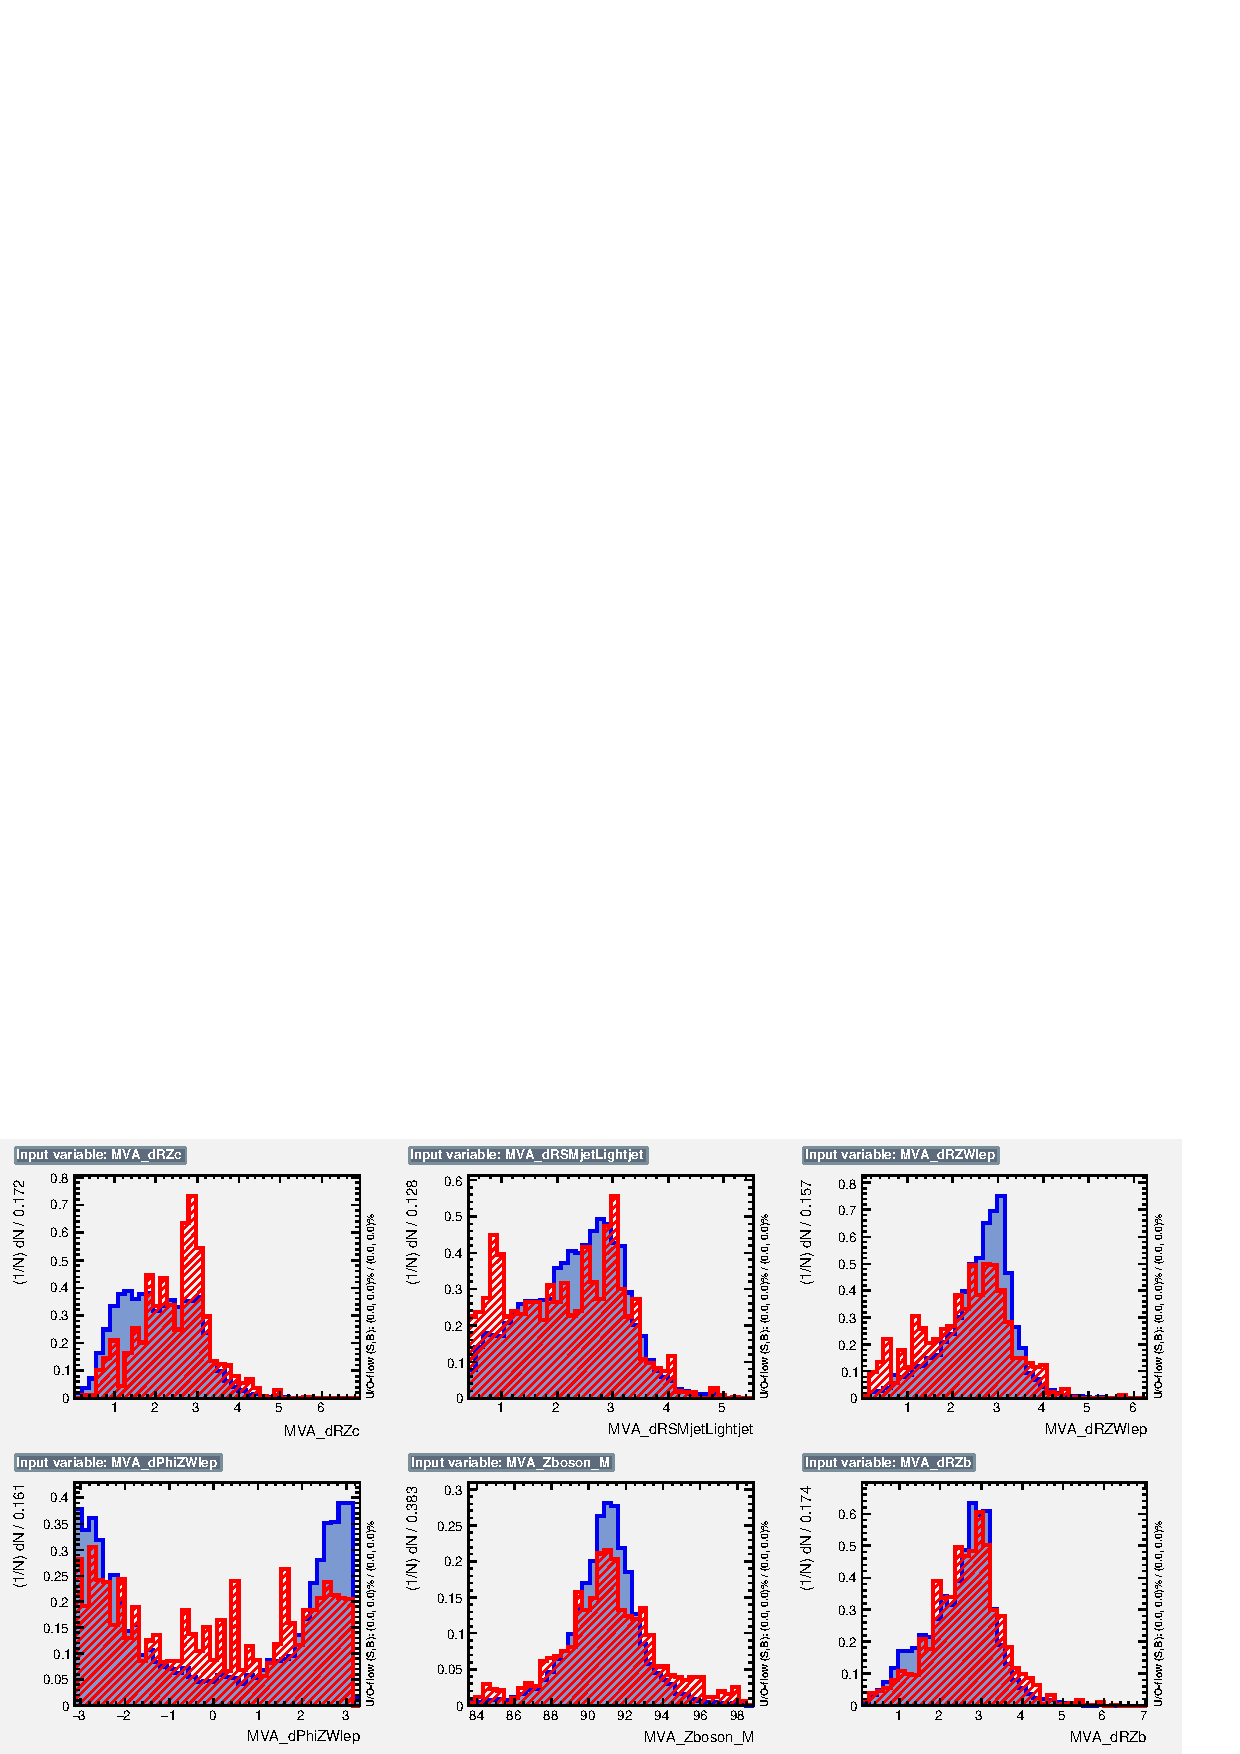
\includegraphics[width=0.48\textwidth]{6_Search/Figures/MVAtechnics/toppairzct/eee/variables_id_c2.png}
	\caption{\eee\ channel. \TTSR: \Zct\ vertex }
	\label{image:Figures3etoppairzct}
\end{figure}

\begin{figure}[htbp]
	\includegraphics[width=0.48\textwidth]{6_Search/Figures/MVAtechnics/toppairzct/eeu/CorrelationMatrixB.png}
	\includegraphics[width=0.48\textwidth]{6_Search/Figures/MVAtechnics/toppairzct/eeu/CorrelationMatrixS.png}
	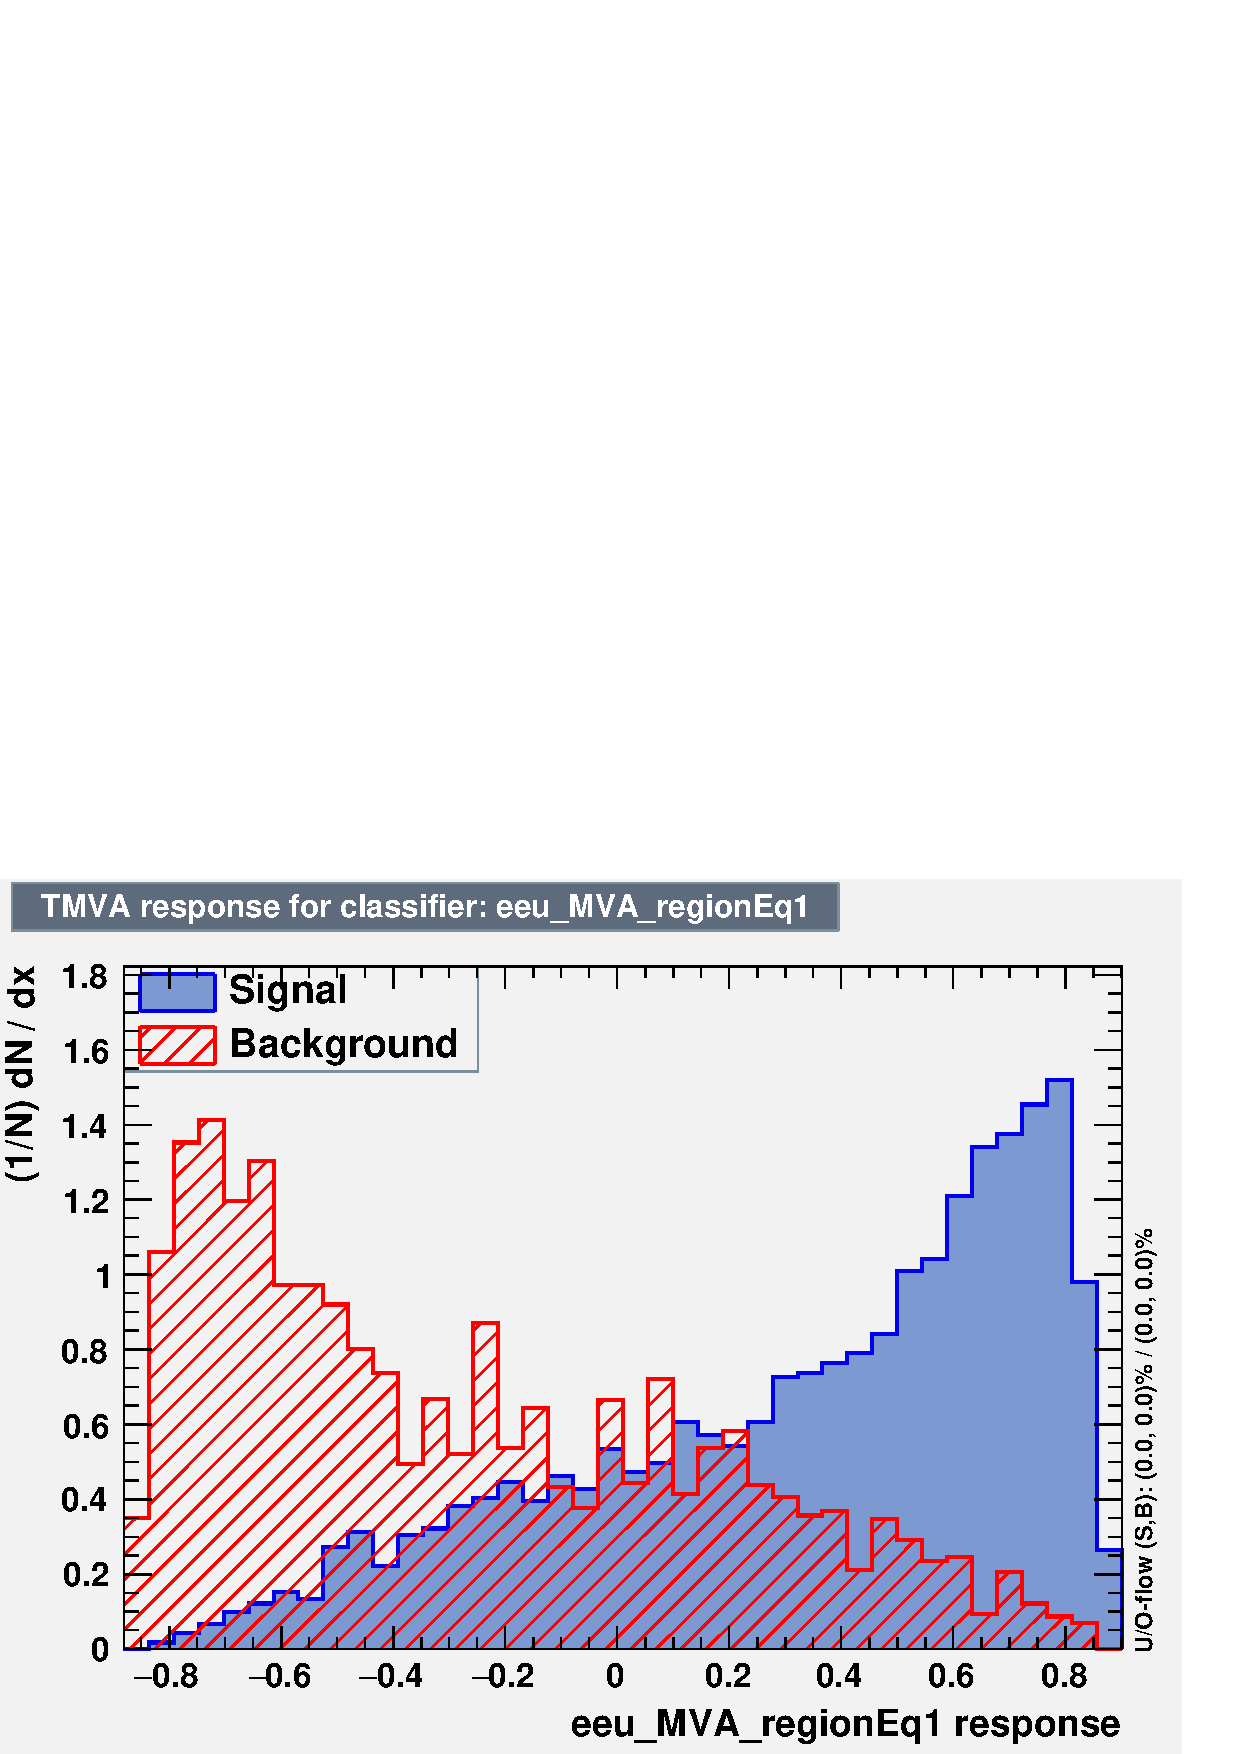
\includegraphics[width=0.48\textwidth]{6_Search/Figures/MVAtechnics/toppairzct/eeu/mva_eeu_MVA_regionEq1.png}
	\includegraphics[width=0.48\textwidth]{6_Search/Figures/MVAtechnics/toppairzct/eeu/rejBvsS.png}
	\includegraphics[width=0.48\textwidth]{6_Search/Figures/MVAtechnics/toppairzct/eeu/variables_id_c1.png}
	\includegraphics[width=0.48\textwidth]{6_Search/Figures/MVAtechnics/toppairzct/eeu/variables_id_c2.png}
	\caption{\eemu\ channel. \TTSR: \Zct\ vertex }
	\label{image:Figureseeutoppairzct}
\end{figure}


\begin{figure}[htbp]
	\includegraphics[width=0.48\textwidth]{6_Search/Figures/MVAtechnics/toppairzct/uue/CorrelationMatrixB.png}
	\includegraphics[width=0.48\textwidth]{6_Search/Figures/MVAtechnics/toppairzct/uue/CorrelationMatrixS.png}
	\includegraphics[width=0.48\textwidth]{6_Search/Figures/MVAtechnics/toppairzct/uue/mva_uue_MVA_regionEq1.png}
	\includegraphics[width=0.48\textwidth]{6_Search/Figures/MVAtechnics/toppairzct/uue/rejBvsS.png}
	\includegraphics[width=0.48\textwidth]{6_Search/Figures/MVAtechnics/toppairzct/uue/variables_id_c1.png}
	\includegraphics[width=0.48\textwidth]{6_Search/Figures/MVAtechnics/toppairzct/uue/variables_id_c2.png}
	\caption{\emumu\ channel. \TTSR: \Zct\ vertex }
	\label{image:Figuresuuetoppairzct}
\end{figure}


\begin{figure}[htbp]
	\includegraphics[width=0.48\textwidth]{6_Search/Figures/MVAtechnics/toppairzct/uuu/CorrelationMatrixB.png}
	\includegraphics[width=0.48\textwidth]{6_Search/Figures/MVAtechnics/toppairzct/uuu/CorrelationMatrixS.png}
	\includegraphics[width=0.48\textwidth]{6_Search/Figures/MVAtechnics/toppairzct/uuu/mva_uuu_MVA_regionEq1.png}
	\includegraphics[width=0.48\textwidth]{6_Search/Figures/MVAtechnics/toppairzct/uuu/rejBvsS.png}
	\includegraphics[width=0.48\textwidth]{6_Search/Figures/MVAtechnics/toppairzct/uuu/variables_id_c1.png}
	\includegraphics[width=0.48\textwidth]{6_Search/Figures/MVAtechnics/toppairzct/uuu/variables_id_c2.png}
	\caption{\mumumu\ channel. \TTSR: \Zct\ vertex }
	\label{image:Figuresuuutoppairzct}
\end{figure}

\begin{figure}[htbp]
	\includegraphics[width=0.48\textwidth]{6_Search/Figures/MVAtechnics/toppairzut/eee/CorrelationMatrixB.png}
	\includegraphics[width=0.48\textwidth]{6_Search/Figures/MVAtechnics/toppairzut/eee/CorrelationMatrixS.png}
	\includegraphics[width=0.48\textwidth]{6_Search/Figures/MVAtechnics/toppairzut/eee/mva_eee_MVA_regionEq1.png}
	\includegraphics[width=0.48\textwidth]{6_Search/Figures/MVAtechnics/toppairzut/eee/rejBvsS.png}
	\includegraphics[width=0.48\textwidth]{6_Search/Figures/MVAtechnics/toppairzut/eee/variables_id_c1.png}
	\includegraphics[width=0.48\textwidth]{6_Search/Figures/MVAtechnics/toppairzut/eee/variables_id_c2.png}
	\caption{\eee\ channel. \TTSR: \Zut\ vertex }
	\label{image:Figureseeetoppairzut}
\end{figure}

\begin{figure}[htbp]
	\includegraphics[width=0.48\textwidth]{6_Search/Figures/MVAtechnics/toppairzut/eeu/CorrelationMatrixB.png}
	\includegraphics[width=0.48\textwidth]{6_Search/Figures/MVAtechnics/toppairzut/eeu/CorrelationMatrixS.png}
	\includegraphics[width=0.48\textwidth]{6_Search/Figures/MVAtechnics/toppairzut/eeu/mva_eeu_MVA_regionEq1.png}
	\includegraphics[width=0.48\textwidth]{6_Search/Figures/MVAtechnics/toppairzut/eeu/rejBvsS.png}
	\includegraphics[width=0.48\textwidth]{6_Search/Figures/MVAtechnics/toppairzut/eeu/variables_id_c1.png}
	\includegraphics[width=0.48\textwidth]{6_Search/Figures/MVAtechnics/toppairzut/eeu/variables_id_c2.png}
	\caption{\eemu\ channel. \TTSR: \Zut\ vertex }
	\label{image:Figureseeutoppairzut}
\end{figure}


\begin{figure}[htbp]
	\includegraphics[width=0.48\textwidth]{6_Search/Figures/MVAtechnics/toppairzut/uue/CorrelationMatrixB.png}
	\includegraphics[width=0.48\textwidth]{6_Search/Figures/MVAtechnics/toppairzut/uue/CorrelationMatrixS.png}
	\includegraphics[width=0.48\textwidth]{6_Search/Figures/MVAtechnics/toppairzut/uue/mva_uue_MVA_regionEq1.png}
	\includegraphics[width=0.48\textwidth]{6_Search/Figures/MVAtechnics/toppairzut/uue/rejBvsS.png}
	\includegraphics[width=0.48\textwidth]{6_Search/Figures/MVAtechnics/toppairzut/uue/variables_id_c1.png}
	\includegraphics[width=0.48\textwidth]{6_Search/Figures/MVAtechnics/toppairzut/uue/variables_id_c2.png}
	\caption{\emumu\ channel. \TTSR: \Zut\ vertex }
	\label{image:Figuresuuetoppairzut}
\end{figure}


\begin{figure}[htbp]
	\includegraphics[width=0.48\textwidth]{6_Search/Figures/MVAtechnics/toppairzut/uuu/CorrelationMatrixB.png}
	\includegraphics[width=0.48\textwidth]{6_Search/Figures/MVAtechnics/toppairzut/uuu/CorrelationMatrixS.png}
	\includegraphics[width=0.48\textwidth]{6_Search/Figures/MVAtechnics/toppairzut/uuu/mva_uuu_MVA_regionEq1.png}
	\includegraphics[width=0.48\textwidth]{6_Search/Figures/MVAtechnics/toppairzut/uuu/rejBvsS.png}
	\includegraphics[width=0.48\textwidth]{6_Search/Figures/MVAtechnics/toppairzut/uuu/variables_id_c1.png}
	\includegraphics[width=0.48\textwidth]{6_Search/Figures/MVAtechnics/toppairzut/uuu/variables_id_c2.png}
	\caption{\mumumu\ channel. \TTSR: \Zut\ vertex }
	\label{image:Figuresuuutoppairzut}
\end{figure}

\begin{figure}[htbp]
	\includegraphics[width=0.48\textwidth]{6_Search/Figures/MVAtechnics/singletopzct/eee/CorrelationMatrixB.png}
	\includegraphics[width=0.48\textwidth]{6_Search/Figures/MVAtechnics/singletopzct/eee/CorrelationMatrixS.png}
	\includegraphics[width=0.48\textwidth]{6_Search/Figures/MVAtechnics/singletopzct/eee/mva_eee_MVA_regionEq0.png}
	\includegraphics[width=0.48\textwidth]{6_Search/Figures/MVAtechnics/singletopzct/eee/rejBvsS.png}
	\includegraphics[width=0.48\textwidth]{6_Search/Figures/MVAtechnics/singletopzct/eee/variables_id_c1.png}
	%	\includegraphics[width=0.48\textwidth]{6_Search/Figures/MVAtechnics/singletopzct/eee/variables_id_c2.png}
	\caption{\eee\ channel. \STSR: \Zct\ vertex }
	\label{image:Figures3esingletopzct}
\end{figure}

\begin{figure}[htbp]
	\includegraphics[width=0.48\textwidth]{6_Search/Figures/MVAtechnics/singletopzct/eeu/CorrelationMatrixB.png}
	\includegraphics[width=0.48\textwidth]{6_Search/Figures/MVAtechnics/singletopzct/eeu/CorrelationMatrixS.png}
	\includegraphics[width=0.48\textwidth]{6_Search/Figures/MVAtechnics/singletopzct/eeu/mva_eeu_MVA_regionEq0.png}
	\includegraphics[width=0.48\textwidth]{6_Search/Figures/MVAtechnics/singletopzct/eeu/rejBvsS.png}
	\includegraphics[width=0.48\textwidth]{6_Search/Figures/MVAtechnics/singletopzct/eeu/variables_id_c1.png}
	%	\includegraphics[width=0.48\textwidth]{6_Search/Figures/MVAtechnics/singletopzct/eeu/variables_id_c2.png}
	\caption{\eemu\ channel. \STSR: \Zct\ vertex }
	\label{image:Figureseeusingletopzct}
\end{figure}


\begin{figure}[htbp]
	\includegraphics[width=0.48\textwidth]{6_Search/Figures/MVAtechnics/singletopzct/uue/CorrelationMatrixB.png}
	\includegraphics[width=0.48\textwidth]{6_Search/Figures/MVAtechnics/singletopzct/uue/CorrelationMatrixS.png}
	\includegraphics[width=0.48\textwidth]{6_Search/Figures/MVAtechnics/singletopzct/uue/mva_uue_MVA_regionEq0.png}
	\includegraphics[width=0.48\textwidth]{6_Search/Figures/MVAtechnics/singletopzct/uue/rejBvsS.png}
	\includegraphics[width=0.48\textwidth]{6_Search/Figures/MVAtechnics/singletopzct/uue/variables_id_c1.png}
	%	\includegraphics[width=0.48\textwidth]{6_Search/Figures/MVAtechnics/singletopzct/uue/variables_id_c2.png}
	\caption{\emumu\ channel. \STSR: \Zct\ vertex }
	\label{image:Figuresuuesingletopzct}
\end{figure}


\begin{figure}[htbp]
	\includegraphics[width=0.48\textwidth]{6_Search/Figures/MVAtechnics/singletopzct/uuu/CorrelationMatrixB.png}
	\includegraphics[width=0.48\textwidth]{6_Search/Figures/MVAtechnics/singletopzct/uuu/CorrelationMatrixS.png}
	\includegraphics[width=0.48\textwidth]{6_Search/Figures/MVAtechnics/singletopzct/uuu/mva_uuu_MVA_regionEq0.png}
	\includegraphics[width=0.48\textwidth]{6_Search/Figures/MVAtechnics/singletopzct/uuu/rejBvsS.png}
	\includegraphics[width=0.48\textwidth]{6_Search/Figures/MVAtechnics/singletopzct/uuu/variables_id_c1.png}
	%	\includegraphics[width=0.48\textwidth]{6_Search/Figures/MVAtechnics/singletopzct/uuu/variables_id_c2.png}
	\caption{\mumumu\ channel. \STSR: \Zct\ vertex }
	\label{image:Figuresuuusingletopzct}
\end{figure}

\begin{figure}[htbp]
	\includegraphics[width=0.48\textwidth]{6_Search/Figures/MVAtechnics/singletopzut/eee/CorrelationMatrixB.png}
	\includegraphics[width=0.48\textwidth]{6_Search/Figures/MVAtechnics/singletopzut/eee/CorrelationMatrixS.png}
	\includegraphics[width=0.48\textwidth]{6_Search/Figures/MVAtechnics/singletopzut/eee/mva_eee_MVA_regionEq0.png}
	\includegraphics[width=0.48\textwidth]{6_Search/Figures/MVAtechnics/singletopzut/eee/rejBvsS.png}
	\includegraphics[width=0.48\textwidth]{6_Search/Figures/MVAtechnics/singletopzut/eee/variables_id_c1.png}
	\includegraphics[width=0.48\textwidth]{6_Search/Figures/MVAtechnics/singletopzut/eee/variables_id_c2.png}
	\caption{\eee\ channel. \STSR: \Zut\ vertex }
	\label{image:Figureseeesingletopzut}
\end{figure}

\begin{figure}[htbp]
	\includegraphics[width=0.48\textwidth]{6_Search/Figures/MVAtechnics/singletopzut/eeu/CorrelationMatrixB.png}
	\includegraphics[width=0.48\textwidth]{6_Search/Figures/MVAtechnics/singletopzut/eeu/CorrelationMatrixS.png}
	\includegraphics[width=0.48\textwidth]{6_Search/Figures/MVAtechnics/singletopzut/eeu/mva_eeu_MVA_regionEq0.png}
	\includegraphics[width=0.48\textwidth]{6_Search/Figures/MVAtechnics/singletopzut/eeu/rejBvsS.png}
	\includegraphics[width=0.48\textwidth]{6_Search/Figures/MVAtechnics/singletopzut/eeu/variables_id_c1.png}
	\includegraphics[width=0.48\textwidth]{6_Search/Figures/MVAtechnics/singletopzut/eeu/variables_id_c2.png}
	\caption{\eemu\ channel. \STSR: \Zut\ vertex }
	\label{image:Figureseeusingletopzut}
\end{figure}


\begin{figure}[htbp]
	\includegraphics[width=0.48\textwidth]{6_Search/Figures/MVAtechnics/singletopzut/uue/CorrelationMatrixB.png}
	\includegraphics[width=0.48\textwidth]{6_Search/Figures/MVAtechnics/singletopzut/uue/CorrelationMatrixS.png}
	\includegraphics[width=0.48\textwidth]{6_Search/Figures/MVAtechnics/singletopzut/uue/mva_uue_MVA_regionEq0.png}
	\includegraphics[width=0.48\textwidth]{6_Search/Figures/MVAtechnics/singletopzut/uue/rejBvsS.png}
	\includegraphics[width=0.48\textwidth]{6_Search/Figures/MVAtechnics/singletopzut/uue/variables_id_c1.png}
	\includegraphics[width=0.48\textwidth]{6_Search/Figures/MVAtechnics/singletopzut/uue/variables_id_c2.png}
	\caption{\emumu\ channel. \STSR: \Zut\ vertex }
	\label{image:Figuresuuesingletopzut}
\end{figure}


\begin{figure}[htbp]
	\includegraphics[width=0.48\textwidth]{6_Search/Figures/MVAtechnics/singletopzut/uuu/CorrelationMatrixB.png}
	\includegraphics[width=0.48\textwidth]{6_Search/Figures/MVAtechnics/singletopzut/uuu/CorrelationMatrixS.png}
	\includegraphics[width=0.48\textwidth]{6_Search/Figures/MVAtechnics/singletopzut/uuu/mva_uuu_MVA_regionEq0.png}
	\includegraphics[width=0.48\textwidth]{6_Search/Figures/MVAtechnics/singletopzut/uuu/rejBvsS.png}
	\includegraphics[width=0.48\textwidth]{6_Search/Figures/MVAtechnics/singletopzut/uuu/variables_id_c1.png}
	\includegraphics[width=0.48\textwidth]{6_Search/Figures/MVAtechnics/singletopzut/uuu/variables_id_c2.png}
	\caption{\mumumu\ channel. \STSR: \Zut\ vertex }
	\label{image:Figuresuuusingletopzut}
\end{figure}
\chapter{Prefit distributions}
\label{app:Prefit}
%\section{BDT input variables}
%\label{app:BDTdis}
\section{BDT distributions}
\label{app:BDT}
\begin{figure}[htbp]
	\centering
	\includegraphics[width=0.49\linewidth]{6_Search/Figures/BDTdistributions/toppair_Zut_BDT_all_Stack}
	\includegraphics[width=0.49\linewidth]{6_Search/Figures/BDTdistributions/toppair_Zct_BDT_all_Stack}
	\includegraphics[width=0.49\linewidth]{6_Search/Figures/BDTdistributions/singletop_Zut_BDT_all_Stack}
	\includegraphics[width=0.49\linewidth]{6_Search/Figures/BDTdistributions/singletop_Zct_BDT_all_Stack}
	\caption{Distributions of the discriminating variable before the fit, all different leptonic channels together. Upper left: \TTSR: \Zut\ vertex , upper right: \TTSR: \Zct\ vertex ; lower left: \STSR: \Zut\ vertex , lower right: \STSR: \Zct\ vertex .}
	\label{fig:bdtallstack}
\end{figure}	

\begin{figure}[ht]
	\centering
	\includegraphics[width=0.49\linewidth]{6_Search/Figures/BDTdistributions/toppair_Zut_BDT_uuu_Stack}
	\includegraphics[width=0.49\linewidth]{6_Search/Figures/BDTdistributions/toppair_Zct_BDT_uuu_Stack}
	\includegraphics[width=0.49\linewidth]{6_Search/Figures/BDTdistributions/singletop_Zut_BDT_uuu_Stack}
	\includegraphics[width=0.49\linewidth]{6_Search/Figures/BDTdistributions/singletop_Zct_BDT_uuu_Stack}
	\caption{Distributions of the discriminating variable before the fit, \mumumu\  channel. Upper left: \TTSR: \Zut\ vertex , upper right: \TTSR: \Zct\ vertex ; lower left: \STSR: \Zut\ vertex , lower right: \STSR: \Zct\ vertex .}
	\label{fig:bdtuuustack}
\end{figure}


\begin{figure}[ht]
	\centering
	\includegraphics[width=0.39\linewidth]{6_Search/Figures/BDTdistributions/toppair_Zut_BDT_uue_Stack}
	\includegraphics[width=0.39\linewidth]{6_Search/Figures/BDTdistributions/toppair_Zct_BDT_uue_Stack}
	\includegraphics[width=0.39\linewidth]{6_Search/Figures/BDTdistributions/singletop_Zut_BDT_uue_Stack}
	\includegraphics[width=0.39\linewidth]{6_Search/Figures/BDTdistributions/singletop_Zct_BDT_uue_Stack}
	\caption{Distributions of the discriminating variable before the fit, \emumu\  channel. Upper left: \TTSR: \Zut\ vertex , upper right: \TTSR: \Zct\ vertex ; lower left: \STSR: \Zut\ vertex , lower right: \STSR: \Zct\ vertex .}
	\label{fig:bdtuuestack}
\end{figure}

\begin{figure}[ht]
	\centering
	\includegraphics[width=0.39\linewidth]{6_Search/Figures/BDTdistributions/toppair_Zut_BDT_eeu_Stack}
	\includegraphics[width=0.39\linewidth]{6_Search/Figures/BDTdistributions/toppair_Zct_BDT_eeu_Stack}
	\includegraphics[width=0.39\linewidth]{6_Search/Figures/BDTdistributions/singletop_Zut_BDT_eeu_Stack}
	\includegraphics[width=0.39\linewidth]{6_Search/Figures/BDTdistributions/singletop_Zct_BDT_eeu_Stack}
	\caption{Distributions of the discriminating variable before the fit, \eemu\  channel. Upper left: \TTSR: \Zut\ vertex , upper right: \TTSR: \Zct\ vertex ; lower left: \STSR: \Zut\ vertex , lower right: \STSR: \Zct\ vertex .}
	\label{fig:bdteeustack}
\end{figure}



\begin{figure}[ht]
	\centering
	\includegraphics[width=0.39\linewidth]{6_Search/Figures/BDTdistributions/toppair_Zut_BDT_eee_Stack}
	\includegraphics[width=0.39\linewidth]{6_Search/Figures/BDTdistributions/toppair_Zct_BDT_eee_Stack}
	\includegraphics[width=0.39\linewidth]{6_Search/Figures/BDTdistributions/singletop_Zut_BDT_eee_Stack}
	\includegraphics[width=0.39\linewidth]{6_Search/Figures/BDTdistributions/singletop_Zct_BDT_eee_Stack}
	\caption{Distributions of the discriminating variable before the fit, \eee\  channel. Upper left: \TTSR: \Zut\ vertex , upper right: \TTSR: \Zct\ vertex ; lower left: \STSR: \Zut\ vertex , lower right: \STSR: \Zct\ vertex .}
	\label{fig:bdteeestack}
\end{figure}
\clearpage
\section{Transverse W boson mass distributions}
\label{app:MTW}
\begin{figure}[htbp]
	\centering
	\includegraphics[width=0.49\linewidth]{6_Search/Figures/MTWstack/AllBkg/MTW_all_Stack}
	\caption{Distributions of the transverse mass of the \PW\ boson before the fit, all different leptonic channels together. Upper left: \TTSR: \Zut\ vertex , upper right: \TTSR: \Zct\ vertex ; lower left: \STSR: \Zut\ vertex , lower right: \STSR: \Zct\ vertex .}
	\label{fig:mtwallstack}
\end{figure}
\begin{figure}[htbp]
	\centering
	\includegraphics[width=0.49\linewidth]{6_Search/Figures/MTWstack/AllBkg/MTW_uuu_Stack}
	\includegraphics[width=0.49\linewidth]{6_Search/Figures/MTWstack/AllBkg/MTW_uue_Stack}
	\includegraphics[width=0.49\linewidth]{6_Search/Figures/MTWstack/AllBkg/MTW_eeu_Stack}
	\includegraphics[width=0.49\linewidth]{6_Search/Figures/MTWstack/AllBkg/MTW_eee_Stack}
	\caption{Distributions of the transverse mass of the \PW\ boson before the fit, all different leptonic channels together. Upper left: \TTSR: \Zut\ vertex , upper right: \TTSR: \Zct\ vertex ; lower left: \STSR: \Zut\ vertex , lower right: \STSR: \Zct\ vertex .}
	\label{fig:mtwallstac}
\end{figure}
\clearpage
\section{Input variables of the BDT}
\label{app:prefitBDTvar}
\begin{figure}[htbp]
	\centering
	\includegraphics[width=0.25\linewidth]{6_Search/Figures/BDTinputvars/Zut/Stack/toppair_MVA_SMtop_Eta_all_Stack}
	\includegraphics[width=0.25\linewidth]{6_Search/Figures/BDTinputvars/Zut/Stack/toppair_MVA_mlb_all_Stack}
	\includegraphics[width=0.25\linewidth]{6_Search/Figures/BDTinputvars/Zut/Stack/toppair_MVA_dPhiWlepb_all_Stack}
	\includegraphics[width=0.25\linewidth]{6_Search/Figures/BDTinputvars/Zut/Stack/toppair_MVA_deltaRWlepJet_min_all_Stack}
	\includegraphics[width=0.25\linewidth]{6_Search/Figures/BDTinputvars/Zut/Stack/toppair_MVA_Zboson_M_all_Stack}
	\includegraphics[width=0.25\linewidth]{6_Search/Figures/BDTinputvars/Zut/Stack/toppair_MVA_dPhiZWlep_all_Stack}
	\includegraphics[width=0.25\linewidth]{6_Search/Figures/BDTinputvars/Zut/Stack/toppair_MVA_dRWlepb_all_Stack}
	\includegraphics[width=0.25\linewidth]{6_Search/Figures/BDTinputvars/Zut/Stack/toppair_MVA_NJets_CSVv2M_all_Stack}
	\includegraphics[width=0.25\linewidth]{6_Search/Figures/BDTinputvars/Zut/Stack/toppair_MVA_FCNCtop_M_all_Stack}
	\includegraphics[width=0.25\linewidth]{6_Search/Figures/BDTinputvars/Zut/Stack/toppair_MVA_dRZc_all_Stack}
	\includegraphics[width=0.25\linewidth]{6_Search/Figures/BDTinputvars/Zut/Stack/toppair_MVA_dRSMjetLightjet_all_Stack}
	\caption{The normalised input variables for reconstructing the multivariate discriminator in the \TTSR\ for the \Zut\ vertex.}
	\label{fig:toppairZutprefitstack}
\end{figure}

\begin{figure}[htbp]
	\centering
	\includegraphics[width=0.25\linewidth]{6_Search/Figures/BDTinputvars/Zut/Stack/singletop_MVA_SMtop_Eta_all_Stack}
	\includegraphics[width=0.25\linewidth]{6_Search/Figures/BDTinputvars/Zut/Stack/singletop_MVA_mlb_all_Stack}
	\includegraphics[width=0.25\linewidth]{6_Search/Figures/BDTinputvars/Zut/Stack/singletop_MVA_dPhiWlepb_all_Stack}
	\includegraphics[width=0.25\linewidth]{6_Search/Figures/BDTinputvars/Zut/Stack/singletop_MVA_dPhiZWlep_all_Stack}
	\includegraphics[width=0.25\linewidth]{6_Search/Figures/BDTinputvars/Zut/Stack/singletop_MVA_dRWlepb_all_Stack}
	\includegraphics[width=0.25\linewidth]{6_Search/Figures/BDTinputvars/Zut/Stack/singletop_MVA_dRWlepb_all_Stack}
	\includegraphics[width=0.25\linewidth]{6_Search/Figures/BDTinputvars/Zut/Stack/singletop_MVA_charge_asym_all_Stack}
	\includegraphics[width=0.25\linewidth]{6_Search/Figures/BDTinputvars/Zut/Stack/singletop_MVA_bdiscCSVv2_jet_0_all_Stack}
	\includegraphics[width=0.25\linewidth]{6_Search/Figures/BDTinputvars/Zut/Stack/singletop_MVA_TotalHt_lep_all_Stack}
	\includegraphics[width=0.25\linewidth]{6_Search/Figures/BDTinputvars/Zut/Stack/singletop_MVA_ptWQ_all_Stack}
	\caption{The normalised input variables for reconstructing the multivariate discriminator in the \STSR\ for the \Zut\ vertex.}
	\label{fig:singletopZutprefitstack}
\end{figure}

\begin{figure}[htbp]
	\centering
%	\includegraphics[width=0.25\linewidth]{6_Search/Figures/BDTinputvars/Zct/Stack/toppair_MVA_mlb_all_Stack}
%	\includegraphics[width=0.25\linewidth]{6_Search/Figures/BDTinputvars/Zct/Stack/toppair_MVA_Zboson_M_all_Stack}
%	\includegraphics[width=0.25\linewidth]{6_Search/Figures/BDTinputvars/Zct/Stack/toppair_MVA_dPhiZWlep_all_Stack}
%	\includegraphics[width=0.25\linewidth]{6_Search/Figures/BDTinputvars/Zct/Stack/toppair_MVA_dRWlepb_all_Stack}
%	\includegraphics[width=0.25\linewidth]{6_Search/Figures/BDTinputvars/Zct/Stack/toppair_MVA_NJets_CSVv2M_all_Stack}
%	\includegraphics[width=0.25\linewidth]{6_Search/Figures/BDTinputvars/Zct/Stack/toppair_MVA_FCNCtop_M_all_Stack}
%	\includegraphics[width=0.25\linewidth]{6_Search/Figures/BDTinputvars/Zct/Stack/toppair_MVA_dRZc_all_Stack}
%	\includegraphics[width=0.25\linewidth]{6_Search/Figures/BDTinputvars/Zct/Stack/toppair_MVA_dRSMjetLightjet_all_Stack}
%	\includegraphics[width=0.25\linewidth]{6_Search/Figures/BDTinputvars/Zct/Stack/toppair_MVA_TotalInvMass_all_Stack}
%	\includegraphics[width=0.25\linewidth]{6_Search/Figures/BDTinputvars/Zct/Stack/toppair_MVA_dRZWlep_all_Stack}
%	\includegraphics[width=0.25\linewidth]{6_Search/Figures/BDTinputvars/Zct/Stack/toppair_MVA_Bdis_Lightjet_all_Stack}
%	\includegraphics[width=0.25\linewidth]{6_Search/Figures/BDTinputvars/Zct/Stack/toppair_MVA_dRZb_all_Stack}
	\caption{The normalised input variables for reconstructing the multivariate discriminator in the \TTSR\ for the \Zct\ vertex.}
	\label{fig:toppairZctprefitstack}
\end{figure}

\begin{figure}[htbp]
	\centering
%	\includegraphics[width=0.25\linewidth]{6_Search/Figures/BDTinputvars/Zct/Stack/singletop_MVA_SMtop_Eta_all_Stack}
%	\includegraphics[width=0.25\linewidth]{6_Search/Figures/BDTinputvars/Zct/Stack/singletop_MVA_mlb_all_Stack}
%	\includegraphics[width=0.25\linewidth]{6_Search/Figures/BDTinputvars/Zct/Stack/singletop_MVA_dPhiWlepb_all_Stack}
%	\includegraphics[width=0.25\linewidth]{6_Search/Figures/BDTinputvars/Zct/Stack/singletop_MVA_bdiscCSVv2_jet_0_all_Stack}
%	\includegraphics[width=0.25\linewidth]{6_Search/Figures/BDTinputvars/Zct/Stack/singletop_MVA_TotalInvMass_lep_all_Stack}
%	\includegraphics[width=0.25\linewidth]{6_Search/Figures/BDTinputvars/Zct/Stack/singletop_MVA_dRZWlep_all_Stack}   
	\caption{The normalised input variables for reconstructing the multivariate discriminator in the \STSR\ for the \Zct\ vertex.}
	\label{fig:singletopZctprefitstack}
\end{figure}


\chapter{Limit setting validations}
\section{Blinded initial fit, postfit distributions}
\label{app:IniFitDis}

\clearpage
\section{Post fit distributions of the BDT input vars}
\label{app:PostFit}